\label{spdm}
The term ``simplified process design methods'' is used here to describe inventory generation methods from literature (\cite{Parvatker.2019, Hischier.2005, Perry.1999, Smith.2017, JimenezGonzalez.2000}), that are based on chemical process engineering, but rely on little data input for calculation.

The goal of this chapter is to qualitatively understand the influence of using \acl{spdm}s on inventory components and on selected impact categories. A generic model of chemical processes reveals which inventory components are relevant in context of chemical processes. Later, this thesis introduces and evaluates \acl{spdm}s to calculate inventories for chemical unit processes. The results of the evaluation are summarized in Table \ref{tab:spdm}, at the end of the chapter.

\section{Simplified Model of Chemical Processes}
\label{simplified-model-processes}
To assess which inventory components enter and leave the system of a chemical process, a simplified model of chemical processes is used. %Later, in chapter \ref{analysis-spdm}, the \acl{spdm}s are presented and analysed with regard to generating the inventory components.
Also, the case study in chapter \ref{chap:case study} is calculated on the basis of the simplified model of chemical processes.

%Figure: Flow Sheet
\begin{figure}[htp]
        \centering
        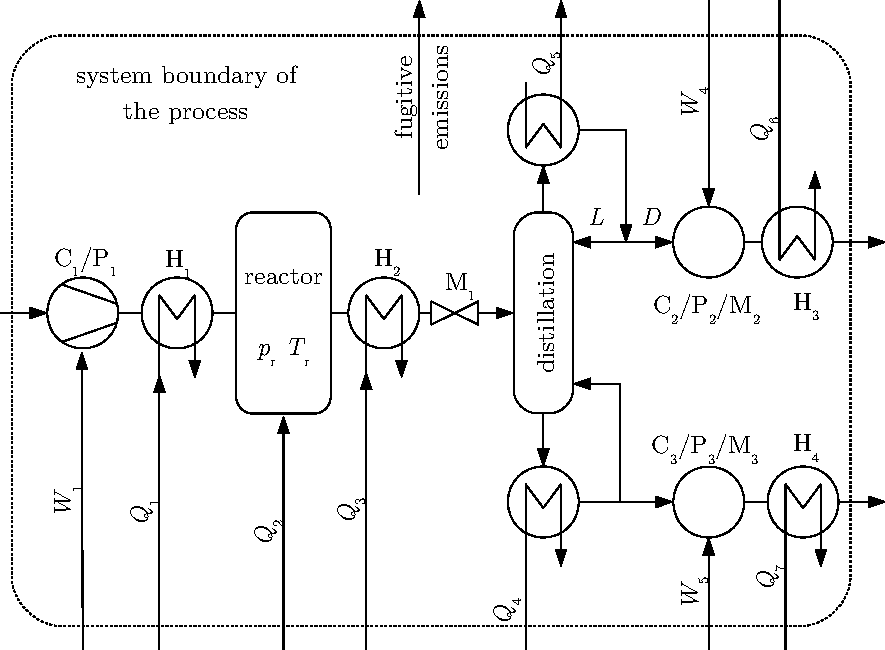
\includegraphics[width=\textwidth]{images/flow_sheet.pdf}
        \caption[Generic flow sheet]{Generic flow sheet: This flow sheet illustrates how chemical processes are simplified in this thesis. $p_r$ and $T_r$ are reaction pressure and temperature, C$_i$ are compressors, P$_i$ pumps and M$_i$ chokes, H$_i$ are heat exchangers, $L$ is the reflux flow, $D$ the distillate flow, $W_i$ are electrical works and $Q_i$ are heat flows.}
        \label{fig:flow sheet}
\end{figure}

\paragraph{Industrial chemical processes}
In general, industrial chemical processes comprise a complex network of chemical engineering operations: a heat exchangers network, several reactors, pumps, compressors, distillation columns, filters, dryers and chokes. 

\paragraph{Flow sheet}To describe the sequence of operations in chemical processes, flow sheets were developed. Flow sheets show all process equipment and how it is interconnected. Designing the flow sheet of industrial chemical processes is the field of process design engineers and requires a large amount of resources, such as time and knowledge. Every chemical process has its own flow sheet  \cite{Douglas.1985}. 

For the generation of inventory data of chemical processes, it is essential to know the sequence of unit processes. Thus, the flow sheet is the basis for later calculation of inventory data.  

\paragraph{Generic flow sheet} Because industrial processes have unique flow sheets and the automated generation of flow sheets is challenging, this thesis uses a simplified generic flow sheet for generating LCA databases. Figure \ref{fig:flow sheet} illustrates this generic flow sheet. The generic flow sheet considers the minimum equipment to perform chemical reactions: heat exchangers, compressor/pumps, one reactor and one distillation column.

On the left side of the flow sheet, educts enter the chemical process. The educts are first compressed to reaction pressure. For gaseous educts, the compression is done by the compressor C$_1$; for liquid educts by the pump P$_1$. Compressor or pump are driven by mechanical work $W_1$, which is ether supplied by a turbine, engine or electric motor. The compressor is followed by the heat exchanger H$_1$ that conditions the educts to reaction temperature. To change the temperature, heat $Q_1$ is introduced. In the next step, the educts pass the reactor and convert partially at reaction condition ($p_r$ and $T_r$). For endothermic reaction, heat $Q_2$ has to be introduced to maintain reaction temperature $(Q_2>0)$, exothermic reactions release heat that has to be dissipated $(Q_2<0)$. According to Douglas \cite{Douglas.1985}, industrial reactors have an educt recycling loop: unreacted educts are separated and feed back into the entrance of the reactor. In this thesis, it is assumed that the industrial reactor, separator of unreacted educts and recycling loop is replaced by the generic reactor. The generic reactor lacks the educt recycling, however considers the effect of the educt recycling by a higher conversion. Nevertheless, the generic reactor outputs unreacted educts and non-products, which are considered as waste. The heat exchanger H$_2$ and the choke M$_1$ follow, which bring the reactor outlet mixture to distillation conditions. The heat exchanger is supplied with heat $Q_3$. The choke is assumed to be adiabatic here. In the distillation column, the product is separated from waste. To perform the distillation, $Q_4$ is introduced at the bottom of the distillation column and $Q_5$ is dissipated at the top. After the distillation column, the choke M$_2$, the compressor C$_2$ or the pump P$_2$ brings the product to atmospheric pressure. A choke is used if distillation pressure is higher than atmospheric pressure, otherwise a compressor or pump is used. To run the compressors or pumps, the work $W_4$ is necessary. Consecutively, the heat exchanger H$_3$ brings the product to standard temperature. The bottom output of the distillation is ether a second product, waste or a mixture, which is separated in a second distillation column. In the case of a product or waste, the compressor C$_3$, the pump P$_3$ or the choke M$_3$ ensure that the flow leaves the system at atmospheric pressure. The heat exchanger H$_4$ brings the flow to standard temperature.  To keep the overview, fugitive emission sources are unlocated in the flow sheet; all equipment with leakages can emit fugitive emissions. 

%\paragraph{Limitations}The simplified model has limitations of products. For instance, the extracrion of salts from water need crystalization. As there is no crystalizer in the generic flowsheet, salt production cannot be modeled. Due to the above simplifications regarding the number of equipment, there are uncertainties of transferring results obtained from the simplified model to industrial processes.

\paragraph{Inventory components}The inventory of the generic chemical process is a list of flows, which cross the system boundary. In the generic flow sheet (Figure \ref{fig:flow sheet}), mass flows of educts, the product, fugitive emissions as well as flows of work $W_i$ and heat $Q_i$ cross the system boundary. In this thesis, four categories of inventory components are introduced: 
\begin{itemize}
    \item Mass flows are the flows of educt, products and waste;
    \item Electricity, as it is assumed that electricity provides work $W_i$;  
    \item Steam, fuel and other sources of heat are aggregated as heat;
    \item Emissions of substances from equipment leakages are summarized as fugitive emissions.
\end{itemize}

\section{Simplified Life Cycle Impact Assessment Methodology}
\label{chap:lcia-meth}
Chapter \ref{analysis-spdm} evaluates qualitatively how \aclp{spdm} influence the life cycle impact of chemicals. Initially, \aclp{spdm} calculate the inventory. To generate qualitative life cycle impacts from the inventory a simplified LCIA methodology is introduced. Two impact categories are chosen: global warming impact and toxicity. %Yet, Calvo-Serrano et al. found that the impact category ``cumulative energy demand'' is correlated with global warming impact \cite{CalvoSerrano.2018}. Thus, in the following considerations, global warming impact also represents the cumulative energy demand.
The assignment from inventory components to life cycle impacts is:
\begin{itemize}
    \item Electricity and heat: according to the US Energy Information Agency \cite{U.S.EnergyInformationAdministration.202003}, in 2019,  63\% of the energy consumed by the industrial sector in the US was generated by fossil fuels. Due to the fact that the production of heat and electricity from fossil fuels emits CO$_2$, electricity and steam contribute to the global warming impact in this LCIA methodology.
    
    Similarly, the burning of  fossil fuels emits toxic substances \cite{FitzGerald.}. Thus, energy production contributes to the toxicity impact in this simplified LCIA method.
    \item Fugitive emissions: it is assumed that the mass flows within a process are toxic. Therefore, leakages emit traces of toxic substances into the environment. Thus, mass flows contribute to toxicity impacts.
    \item Mass flows: input materials for chemical processes are products of previous chemical processes. The previous processes are burdened with global warming and toxicity impacts. %Also waste that is formed in a chemical process is treated, which requires energy and releases emissions. The impacts of the waste treatment are assigned to the chemical process, as waste treatment is a mandatory part of the life cycle.
    Thus, educt mass flows contribute to global warming and toxicity impacts of the process.
\end{itemize}

\section{Analysis of Simplified Process Design Methods}
\label{analysis-spdm}

The goal of this chapter is to introduce \acl{spdm}s from literature and to qualitatively understand the effect of using \aclp{spdm} on inventory components (Chapter \ref{simplified-model-processes}) and on impacts, using the simplified LCIA methodology (Chapter \ref{chap:lcia-meth}). This thesis focuses on the impact categories ``global warming impact'' and ``toxicity''. 


\subsection{Mass Flows based on the Stoichiometric Equation}
\label{stoichiometry}
The stoichiometric method is a widely used \acl{spdm} in the LCA database Ecoinvent: In version 2.0 of the database, more than half of the inventories of chemicals were generated by the stoichiometric method \cite{Althaus.2007}.

Stoichiometry is used to calculate the input and output mass flows of a chemical reactor \cite{Parvatker.2019} (see reactor in flow sheet Figure \ref{fig:flow sheet}). The basis of the calculation is the balanced stoichiometric equation \[ \sum{\nu_i E_i} \rightleftharpoons \sum{\nu_j P_j},\] with educts $E_i$ and products $P_i$ and  the stoichiometric coefficients $\nu_i$. For using this method, besides the stoichiometric equation, the molar masses of all substances of the reaction have to be known. Then, applying a stationary mass balance around the reactor, the masses of educts, products and waste can be calculated. This serves as inventory for the LCA.\\

%The input to the reactor is \[\nu_i mol\] of every educt, the output is \[\nu_j mol\] of every output of process. molar inventory per desired product: inputs:\[\frac{\nu_i{ mol}}{\nu_P{}mol}\] and outputs \[\frac{\nu_j mol}{\nu_P mol}\]ratios reactants, target chemicals, products \cite{pavatker.2019}: combined with molar weight : respective mass flows, 

%The assumption that a chemical reaction that follows the stoichiometric equation is a good assumption, as long a the stoichiometric equation accounts for all possible side reactions at reaction conditions. However, equilibrium reactions do not convert completely. Thus besides the products there are still significant amounts of educt in the reactor output. To obtain more realistic results, it is possible to  
To evaluate the stoichiometric method, a realistic reactor in industry is compared to a stoichiometric reactor. Industrial reactors often do not use educts in the stoichiometric relation. Instead, one educt is used in excess \cite{Piccinno.2016}. Reasons for excess use are less formation of unwanted side products and a faster conversion \cite{Luyben.2000}. Inevitably, the reactor output still contains much of the excess educt and possibly other unreacted educts in case of equilibrium reactions. Thus, the inventory of an  industrial reactor has more educt input and output than the stoichiometric equation suggests. However, chemical plant operators do not waste the unreacted educts. As explained in Chapter \ref{simplified-model-processes}, industrial reactors are followed by an educt recycling. Because of the circulation of unreacted educts in the recycling loop, the unreacted educts are fed back to the reactor. Assuming a perfect educt recycling without waste, all the outputs of the generic reactor are present exactly in the stoichiometric relation. This can also be seen by performing a mass balance around the reactor with educt recycling. 

Because of the complex calculation of the output composition of a realistic reactor with educt recycling, the educt recycling is not illustrated in the flow sheet (Figure \ref{fig:flow sheet}). The effect of educt recycling is modeled through the ideal, generic reactor. The ideal generic reactor in the flow sheet \ref{fig:flow sheet} replaces a realistic reactor plus educt recycling. For the generic reactor, the educt recycling is replaced by the assumption of stoichiometric input and output flows. On the one hand, this consideration justifies the use of the stoichiometric method.\\%  Thus, assuming a high yield for the generic reactor in this thesis is justified. The results of the mass flow a inventory thus should come close to industrial inventories.\\

On the other hand, it is difficult or economically unfeasible  \cite{Douglas.1985} to separate all the unreacted educts. Thus, the educt recycling is incomplete; a part of educts becomes waste. The more educts are wasted, the more the stoichiometric equation underestimates the inventory. This consideration limits the use of the stoichiometric method.

Incorporating a yield  \cite{Parvatker.2019} to the stoichiometric method aims to offset the influence of waste formation in the process. Yield is defined as the ratio of the obtained amount of product and the theoretical, maximal possible amount of product  \cite{Christen.2010}. The implication of using the stoichiometric method with yield highly depends on the certainty of the yield. If the assumed yield is higher than the real yield, an underestimation of material inventory occurs and vice versa. Hischier et al.  \cite{Hischier.2005} suggests to use a yield of 0.95\footnote{In the source \cite{Hischier.2005}, an efficiency of 0.95 is suggested. It is assumed here that efficiency equals yield.}.

In real chemical reactions, additional ancillary materials are present. Examples of ancillary materials are catalysts and solvents. Depending on the process, solvents and catalysts may be recycled, otherwise wasted after use  \cite{Piccinno.2016}. Thus, a contribution for solvent and catalyst supply and waste treatment to the inventory is assumed. However, ancillary materials are omitted in the stoichiometric method, thus the inventory is underestimated. Evaluating the consequences of the underestimation is difficult, because the amount of solvents and catalysts in relation to the product differ with the specific reaction. In addition, the ecological significance of ancillary materials differ. If ancillary materials have an environmental significance, the impact is underestimated. 

As the stoichiometric method does not calculate energy requirements of the reaction, the energy requirement for operating the educt recycling is not considered in the inventory. Thus, the use of the stoichiometric method contributes to an underestimation of the energy demand of the reaction, if the educt recycling is not modeled with another method. 

To summarize the implications of using the stoichiometric method for the generation of material inventories, an underestimation due to the exclusion of waste is expected. Thus, with the simplified LCIA methodology, an underestimation of global warming impact and toxicity is expected. The exclusion of the energy requirement for educt recycling in the stoichiometric method contributes to an underestimated energy requirement of the product. Incorporating a yield $<1$ into the method may correct the underestimation; or may even change the underestimation to an overestimation.

\subsection{Energy Values of the Ecoinvent Approach}
\label{gendorf}
Ecoinvent has established a method for generating the energy inventories and emissions of chemical processes. According to Hischier et al. \cite{Hischier.2005}, the full method also consists of the stoichiometric method. As stoichiometry is subject of chapter \ref{stoichiometry}, this Chapter focuses on the generation of energy inventories and Chapter \ref{gendorf-emission} on emission inventories.

%Applied to the generic flow sheet (Figure \ref{fig:flow sheet}), the energy inventory part of the ``Ecoinvent-method'' estimates the sum of all heat flows $Q_i$ and the sum of all electricity demands $W_i$. Thereby, t
The Ecoinvent-method takes the average electricity and fuel consumption -- used for the production of chemicals -- as default values for the energy inventory.  The average is calculated from the environmental report of the chemical plant in Gendorf, Germany \cite{GendorfChemiepark.2000}. The Gendorf plant produces approximately 1500 chemical products  \cite{Hischier.2005}.

The calculated average values for energy and fuel consumption are used as default values in the inventory of chemicals. It is assumed that the electricity is used to run process auxiliaries and waste water treatment. Thus, the Ecoinvent-method estimates the energy consumption $\sum W_i$ of the pumps or compressors in the generic flow sheet \ref{fig:flow sheet}. Fuels are assumed to deliver heat for preheating of chemicals and for distillation  \cite{Hischier.2005}. Therefore, the Ecoinvent-method approximates the sum of all heat flows $\sum Q_i$.

Approximating the energy demand with default values is a simplification. Therefore, process specific properties are excluded from consideration. Examples for process specific properties that affect the electricity demand are the process pressures.  The fuel consumption, for instance, is influenced by the process specific property, if the reaction is endothermic or exothermic.

To sum up, the default values are an estimation of the energy demand. It is unpredictable whether the default values approximate the real energy consumption properly or  under- or overestimate it. According to the simplified LCIA methodology (Chapter \ref{chap:lcia-meth}), an under- or overestimation of the global warming impact and toxicity is possible.

%between cradle to gate and gate to gate
%Doppelgendorf (Nachschauen in gendorf umwelterklärung energiebedarf und dann mit Ecoinvent paper vergleichen)




\subsection{Heat Requirement of Reaction, based on Reaction Enthalpy}
\label{enthalpy}
The reaction-enthalpy-method is a basic model for the energy requirement of a reactor. In the flow sheet (Figure \ref{fig:flow sheet}), the method calculates the heat $Q_2$. Within the reaction-enthalpy-method, the heat of reaction is taken as an approximation for the heat requirement of the reactor. The heat of reaction can, for instance, be calculated from the heat of formation  \cite{Parvatker.2019}. The heat of formation is material-specific and can be accessed in chemical property tables.

The scope of the reaction-enthalpy-method simplifies the energy requirement or a reactor: reasons for energy consumption are only partly covered. For instance, heat losses and energy for stirring are excluded in the calculation. According to the reaction-enthalpy-method, endothermic reactions result in heat output. The heat is collected with heat recovery, which has a limited efficiency. Percentages of possible heat recovery depend on the temperature of the reactor  \cite{JimenezGonzalez.2000,Branan.2002}. The higher the temperature, the more heat can be recovered.%At low temperatures, usually the energy from the endothermic reaction is dissipated with cooling water.\\

An advantage of the reaction-enthalpy-method is the little data input that is necessary for the calculation. The reaction-enthalpy-method alone underestimates the energy requirement of a reactor, as it excludes reasons for energy requirement. Thus, global warming impact and toxicity are also underestimated.

\subsection{Heat Required for Temperature Change}
\label{heatup}
The  temperature-change method calculates the energy inventory to heat substances from one temperature level to another.  Applied to the generic flow sheet, the temperature-change method calculates energy demand of the heat exchangers H$_i$ in the generic flow sheet (Figure \ref{fig:flow sheet}). To calculate the energy demand, the temperature difference is needed. Also, information about the heat capacity is necessary. According to Piccinno et al. \cite{Piccinno.2016}, the heat demand $Q_i$ is 
\begin{equation}
\label{equ:temper}
    Q_i=mc_p\Delta T,
\end{equation}
with the heated mass $m$, the isobaric heat capacity $c_p$ and the temperature difference $\Delta T$.

According to Baehr et al. \cite{Baehr.2016}, Equation \ref{equ:temper} incorporates the assumption of an ideal fluid with constant heat capacity; additionally, for the case of a liquid, an isobaric heat exchanger. Also, heat losses are excluded of the analysis, but occur in real heat exchangers. These assumptions have to be justified for the application.

If the temperature is decreased in the heat exchanger, it has to be considered that only a fraction of the heat can be recovered for reuse. This especially applies for low temperature  \cite{JimenezGonzalez.2000,Branan.2002}.

Calculating the energy demand of heating is a standard process design task. Thus, this method is supposed to deliver reliable results for energy inventories and its connected impact category global warming impact and toxicity.

When the temperature-change method is applied to the heat exchanger supplied by $Q_1$, it calculates the energy demand to condition the educts from ambient to reaction temperature. Together with the reaction-enthalpy-method (Chapter \ref{enthalpy}), two causes of the energy demand of reactors (reaction enthalpy and condition) are considered. This serves as a basis for energy inventory calculation of reactions in literature \cite{Parvatker.2019}.





\subsection{Heat Requirement of Distillation by Piccinno et al.}
The distillation method by Piccinno et al. calculates the energy requirement to separate one product.  In the generic flow sheet (Figure \ref{fig:flow sheet}), the energy inventory for distillation is represented by the %heat $Q_3=Q_{heat}$ for heat up to distillation temperature and 
heat $Q_4$ at the bottom of the distillation column to vaporize the liquids.  Heat $Q_5$ is dissipated at the top to condense the product and is assumed to be wasted. Piccino et al. \cite{Piccinno.2016} suggest equation \ref{equa:distil} based on the heat of vaporization:

\begin{equation}
\label{equa:distil}
    Q_4=Q_{dist}=\frac{\Delta h_{vap}m_{dist}\cdot(R+1)}{\eta_{heat}-0.1}. %only R
    %Q_{dist}=\frac{Q_{heat}+Q_{vap}\cdot(R+1)}{\eta_{heat}-1}=\frac{c_pm_{mix}(T_{boil}-T_0)+\Delta h_{vap}m_{mix}\cdot(R+1)}{\eta_{heat}-0.1}. %only R
\end{equation}

In Equation \ref{equa:distil}, $Q_{dist}$ is the heat demand of the distillation,  %$c_p$ is the isobaric heat capacity,
$m_{dist}$ is the mass of the distillate, the head product of the distillation, %$T_{boil}-T_0)$ the temperature difference between distillation inlet and reactor outlet, 
and $\Delta h_{vap}$ is the enthalpy of vaporization. %Calculation of the heat demand to reach the boiling point of the mixture follows the method in chapter \ref{heatup} and delivers \(Q_3=Q_{heat}=c_pm_{mix}(T_{boil}-T_0)\). 
Because of the reflux, a part of the head product is condensed and fed back to the distillation column to be reboiled. The amount of fed back product is described by the reflux ratio $R$, which is reflux flow $L$ divided by the distillate flow $D$. To approximate heat losses, the heating efficiency $\eta_{heat}$ is reduced by 10\% in the formula \cite{Piccinno.2016}.%Distillation does only work, if reflux ratio exceeds the minimum reflux ratio ($R\geq R_{min}$). $R_{min}$ is calculated by the Underwood equation \cite{Piccinno.2016} \[R_{min}=\frac{1}{1-\alpha}\left(\frac{x_{LD}}{x_{LF}}-\frac{\alpha (1-X_{LD})}{1-X_{LF}}\right), \]in which $\alpha$ is the relative volatility, and $x_{LD}$ the traget purity of the distillate and $x_{LF}$ the traget  To ensure, that $R>R_{min}$, the factor 1.2 was introduced in formula \ref{equa:distil}.
 
The energy demand to reach a certain distillation pressure is ignored here, as industrial distillation happens usually under ambient pressure. Exceptions are cases with substances with high boiling points (approximately >200\degree C) or very similar boiling points in the reactor outcome. Anyways, the method is initially developed for batch processes  \cite{Piccinno.2016}, which may limit the accuracy for stationary processes.

The method introduced accounts for all important energy demand in distillation: heat of vaporization and heat losses. The method has a low data requirement: the distillation temperature and additional assumptions for the reflux ratio $R$ and the heat efficiency $\eta_{heat}$. The quality of the energy inventory result depends on choices of the last two parameters. For proper parameters, the distillation method by Piccinno et al. is supposed to generate realistic inventories. Inappropriate parameters may result in an over- or underestimation of the energy requirement and consequentially of the global warming impact and toxicity impact.

\subsection{Energy Requirement of Pumps based on Piccinno et al.}
For liquid reaction processes, this method can be applied to approximate the energy requirement of pumps (see pumps P$_i$, flow sheet Figure \ref{fig:flow sheet}). The energy demand of a pump depends on a variety of physical influences: the height difference, the speed difference of the liquid between pump inlet and outlet, the friction in the pipe to the next equipment and the static pressure drop in the equipment after the pump. Piccinno et al. \cite{Piccinno.2016} quantify the energy demand by
\begin{equation}
\label{equ:pump}
    E_{pump}=\frac{m}{\eta_{pump}}\cdot \left( \Delta h_{equip} \ g+\frac{\Delta v^2}{2}+\frac{\Delta p}{\rho}+\frac{\lambda lv^2}{2d}\right).
\end{equation}


The parameters are mass $m$, efficiency of the pump \(\eta_{pump}\), height difference between pump and equipment inlet $\Delta h$,  gravitational constant $g$, difference in speed between pump inlet and outlet $\Delta v$, static pressure drop in the equipment after the pump $\Delta p_{equip}$,  density of the liquid $\rho$, friction factor $\lambda$, length $l$, diameter $d$ of the pipe and speed of the liquid in the pipe $v$.

Unfortunately, many of those parameters are equipment-size-specific and thus difficult to collect in the scope of fast and automated LCA database generation. Also, friction in pipes is not considered in this thesis. Therefore, Equation \ref{equ:pump} can be simplified by assuming friction free flow, no speed difference between inlet and outlet of the pump and no height difference of equipment:

\begin{equation}
\label{equ:pumpsimple}
    E_{pump}=\frac{m}{\eta_{pump}}\cdot\frac{\Delta p}{\rho},
\end{equation}


%On the one hand, the parameters enable a process specific energy inventory of a pump. On the other side, collecting all parameters can be challenging for a LCA database with a vast amount of chemicals.  If parameter data is not available,  \cite{Piccinno.2016} lists default values for a generic process for parameters in the formula which result in an energy demand per transfered mass of\(55 \frac{J}{kg}\) for every pump, finally. This simplification reduces the data intensity. However, with this simplification the energy inventory only accounts for the number of pumps in the process, but not to the pressure drop and the pump efficiency anymore. Thus, the simplification is only partly process specific and thus assumed to be inaccurate.

where $\Delta p_{pump}$ is now the static pressure difference between pump outlet and inlet. Now, all parameters in equation \ref{equ:pumpsimple} can be derived from the generic flow sheet: with a realistic pump efficiency, the energy inventory is expected to be accurate. Thus, the global warming impact and the toxicity are properly approximated.

\subsection{Energy Requirement of Compressors based on Thermodynamic Considerations}
%Perrys Handbook 1999, page 372 / 2471 or 4-36 thermodynamics  \cite{PerryRobertH..1999}
In gas reaction processes, a compressor is used to increase the pressure instead  of a pump  (compressors C$_i$ in the  generic flow sheet Figure \ref{fig:flow sheet}). This method builds on thermodynamic consideration from Perry's Chemical Engineers' Handbook \cite{Perry.1999}: the fluid is assumed to be ideal and the compression is assumed to be isentropic and completely intercooled after each compressor stage. To include dissipation, a compressor efficiency $\eta$ is introduced. Finally, this yields the equation \[P=\frac{n\gamma RT}{\eta\cdot (\gamma -1)}  \left[ \left(\frac{p_2}{p_1}\right)^\frac{\gamma -1}{n\gamma}-1 \right] \cite{Perry.1999}. \]
Values in the formula are: number of compressor stages $n$, heat capacities $\gamma$ (1.4 for air as ideal gas), temperature $T$, pressure $p$, universal gas constant $R=8.314 \frac{J}{mol K}$, index $1$ before the compressor and index $2$ after the last compressor stage.

This method is easily integrated into LCA databases as it only requires few data. The reliability of the result depends on a realistic value for the efficiency of the compressor. Assuming to know an appropriate efficiency value, this formula is an accurate approximation of the energy requirement of a compressor in a chemical process. Thus, the derived impacts ``global warming impact'' and ``toxicity''  are supposed to be accurate.

\subsection{Fugitive Emissions, based on Empirical Findings by Smith et al. \cite{Smith.2017}}
\label{chap:Smith}
Fugitive emissions occur because of leakages in chemical processes. Smith et al. \cite{Smith.2017} have applied findings about equipment leakages from the United States Environmental Protection Agency  \cite{U.S.EnvironmentalProtectionAgency.1995} to generate life cycle inventory data: 
\[E_T= \sum_{i}n_i \cdot f_i \cdot t\] describes the annual fugitive emission. This equation has to be applied on every single chemical in a process. Within the formula, $i$ is the type of fugitive source (equipment), $n_i$ is the quantity of equipment $i$ in the flow sheet, $f_i$ is the emission factor of equipment $i$ in $\frac{kg}{h\cdot source}$ and $t$ is the operation time in hours per year.

Emissions occur in pumps, compressors, valves, connectors, open-end lines, sampling connection and relief valves \cite{Smith.2017}. Pumps and compressors are the only equipment that is present in the flow sheet Figure \ref{fig:flow sheet}. Therefore, applied to the equipment in the generic flow sheet, the Smith-emission-method only calculates emission inventories for pumps and compressors. The emission factors $f_i$ are introduced in Table \ref{tab:emissionSmith}. Emission factors for equipment that is not existent in the flow sheet, can be obtained from Smith et al, 2017 \cite{Smith.2017}.

\begin{table}[h]
\caption[Average emission factors for equipment in the generic flow sheet by Smith et al.]{Average emission factors for equipment in the generic flow sheet by Smith et al. Light liquids have a vapor pressure higher than 0.3 kPa at 20 °C. Heavy liquids have a vapor pressure below 0.3 kPa at 20 °C (adapted from  \cite{U.S.EnvironmentalProtectionAgency.1995,Smith.2017}).}
\label{tab:emissionSmith}
\centering
\begin{tabular}{ccc}
\toprule
\textbf{equipment type} & \textbf{fluid} & \textbf{emission factor $f_i$ in $\frac{\mathrm{kg}}{\mathrm{h}\cdot \mathrm{source}}$} \\ \midrule
pumps & light liquid & 0.0199\\\
{}& heavy liquid & 0.00862\\
compressors & gas & 0.228\\\bottomrule
\end{tabular}
    
\end{table}

The Smith-emission-method only needs basic data: the quantity of compressors or pumps, the categorization of the vapor pressure in high and low and the material inventory to derive the emissions. The low data requirement makes the method suitable for the fast and automated inventory generation for LCA databases. As the method is based on the environmental report of the Environmental Protection Agency, the factors are supposed to be reliable. 

However, the adaptations of the method in this thesis have excluded emissions from valves, connectors, open-end lines, sampling connection and relief valves. %Thus, this method as it is adapted here, only includes compressor and pumps. 
Because of this limited scope, the method is supposed to slightly underestimate the emission inventory. Therefore, generating LCA datasets with this method will result in a slight underestimation of the derived toxicity impact.

\subsection{Fugitive Emissions Factors of the Ecoinvent Method}
\label{gendorf-emission}
The Ecoinvent-method also estimates fugitive emissions, which are depicted at the top of Figure \ref{fig:flow sheet}. Emissions into the air are assumed to be 0.2 \% of the input materials % Emission to water are assumed to be the difference of unreacted educts and air emission, resulting in 4.8\% of input material
 \cite{Hischier.2005, Althaus.2007}.%Although not mentioned in the Ecoinvent report \cite{Hischier.2005}, some of Ecoinvent datasets use an internal waste water treatment that removes 90\% of the emission from the water \cite{Althaus.2007}. Thus, the emissions to water are reduced to  0.02\%. Solid waste formation is assumed insignificant in liquid or gaseous reactions. Thus, Solid waste are not considered.
Using default emission factors does not reflect different equipment. Still, it is a process-specific assumption: high input of toxic substances result in high emission of toxic material inventory. Nevertheless, the Ecoinvent emission method excludes intermediates and products that are present in the process from the inventory.

In order to understand the ability of the Ecoinvent-method to calculate fugitive emission inventories,
the value of the air emission factor has to be evaluated. Therefore, the Ecoinvent emission factor is compared to the empirical emission factors by Smith et al. \cite{Smith.2017} (see Chapter \ref{chap:Smith}, comparison see Table \ref{tab:comp-fugi-Eco} in the Appendix). The result shows that the Ecoinvent emission factor is at least one magnitude higher than the emission factor by Smith et al. As explained in Chapter \ref{chap:Smith}, the Smith-method slightly underestimates fugitive emissions, thus the Ecoinvent-method still overestimates them. In conclusion, with the LCIA methodology in Chapter \ref{chap:lcia-meth}, the toxicity impact is overestimated by the air emissions of the Ecoinvent-method.


\subsection{Fugitive Emissions based on Rule of Thumb by Jiménez-González et al. \cite{JimenezGonzalez.2000}}
Similar to the method by Smith et al., the fugitive emission method by Jiménez-González generates fugitive emission inventories that originate from equipment leakages. Jiménez-González et al. \cite{JimenezGonzalez.2000} proposes a rule of thumb based on expert judgment, see Table \ref{tab:Jimenez}.

\begin{table}[]
\caption{Fugitive emission factors for the entire chemical process, based on a rule of thumb by Jiménez-González et al. (adapted from \cite{JimenezGonzalez.2000}) }
\label{tab:Jimenez}
\centering
   \begin{tabular}{ccc}
   \toprule
    \textbf{fluid} & \textbf{boiling point} & \textbf{emission factor} \\
            & \textbf{at 1013 hPa }&   \\\midrule
    liquids &  $20...60$ °C   &   2 \%\\
            &   $60...120$ °C &   1 \%\\\midrule
    gases   &   $<20$ °C      &   0.5 \%\\\bottomrule
    \end{tabular}
\end{table}
In contrast to the method by Smith et al., the emission factors by Jiménez-González et al. apply for the entire production process instead of single unit operations. Thus, the method calculates the summed emissions of all equipment in the flow sheet (Figure \ref{fig:flow sheet}). In contrast to the Ecoinvent emission method, which only considers the process inputs, the method by Jiménez-González et al. compiles emissions for all substances present in the production process.

Advantageously, the rule of thumb hardly needs data: only the mass flow inventory and the characterization of the fluids according to the boiling points are necessary. Evaluating the method is difficult, as it is based on expert judgement. However, a comparison of the emission factors by  Jiménez-González et al. and by Smith et al. is possible. The comparison reveals that the factors by Jiménez-González et al. are at least one magnitude higher (see Table \ref{tab:comp-fugi} in the Appendix). Assuming a slight underestimation of the method by Smith et al., the method by Jiménez-González still overestimates the emission inventory and the derived toxicity impact.



\subsection{Summary and Conclusion}

%overview spdm methods table
\begin{table}
\caption[Summary of qualitative implications for life cycle inventory  and impact results when using \acl{spdm}s.]{Summary of qualitative implications for life cycle inventory  and impact results when using \acl{spdm}s. Vertical: \acl{spdm}s, horizontal: inventory components and impacts. ``+'' marks an overestimation by the \acl{spdm}, while ``$-$'' marks an underestimation. ``1'' symbols a proper approximation, ``$\emptyset$'' represents that the method does not influence the inventory component or impact. Behind the symbols, a short comment explains the reason for the over- or underestimation. $R$ is the distillation reflux ratio, $\eta$ is a equipment efficiency. The  transformation from inventory data to impact data is described in Chapter \ref{chap:lcia-meth}.\\
*heat considers the sum of steam, fuel and electricity for process heating}
\label{tab:spdm}
\resizebox{\textwidth}{!}{
\begin{tabular}{ccccccc}\toprule

\makecell{simplified process\\ design method} & \makecell{heat*\\input} & \makecell{electricity\\input} & \makecell{mass\\flows}  & \makecell{fugitive\\ emissions}  & \makecell{global warming\\impact} & toxicity \\\midrule

stoichiometry & \makecell{$-$ educt\\recycling\\energy\\demand} & $\emptyset$ & \makecell{$-$ waste\\formation,\\$-$ ancillary\\material} & $\emptyset$ & \makecell{$-$} & \makecell{$-$} \\\midrule

\makecell{stoichiometry,\\yield $<1$} & \makecell{$-$ educt\\recycling\\energy\\demand} & $\emptyset$ & \makecell{$+-$yield,\\$-$ ancillary\\material} & $\emptyset$ & \makecell{$+-$}  & \makecell{$+-$ }\\\hline

\makecell{process\\energy by\\ Ecoinvent} & \multicolumn{2}{c}{\makecell{$+-$ default values}} & $\emptyset$ & $\emptyset$ & \makecell{$+-$} & \makecell{$+-$} \\\midrule

reaction enthalphy & \makecell{$-$ missing\\ heat losses,\\$-$ (exotherm\\ reaction)\\ incomplete\\heat recovery} & $\emptyset$ & $\emptyset$ & $\emptyset$ & \makecell{$-$} & $-$\\\midrule

\makecell{temperature\\change} & \makecell{1 for heating,\\ $-$ heat recovery\\(cooling)} & $\emptyset$ & $\emptyset$ & $\emptyset$ & \makecell{1 for heating,\\ $-$ for cooling} & \makecell{1 for\\heating,\\ $-$ for\\cooling}\\\midrule

distillation & \makecell{$+-$ R,\\$+-\eta_{heat}$}& $\emptyset$ & $\emptyset$ & $\emptyset$ & $+-$ & $+-$ \\\midrule

\makecell{pump} & $\emptyset$ & \makecell{1 for\\proper $\eta$} & $\emptyset$ & $\emptyset$ & \makecell{1 } & 1 \\\midrule

\makecell{compressor} & $\emptyset$ & \makecell{1 for\\proper $\eta$} & $\emptyset$ & $\emptyset$ & 1  & 1 \\\midrule

\makecell{fugitive\\emissions\\by Smith et al.} & $\emptyset$ & $\emptyset$ & $\emptyset$ & $-/1$ & $\emptyset$ &$-/1$\\\midrule

\makecell{fugitive\\emissions by\\Ecoinvent} & $\emptyset$ & $\emptyset$ & $\emptyset$ & \makecell{$+$} & $\emptyset$ & \makecell{$+$} \\\midrule

\makecell{fugitive\\emissions\\by Jiménez-\\González et al.} & $\emptyset$ & $\emptyset$ & $\emptyset$ & + & $\emptyset$ & + \\\bottomrule 

\end{tabular}}
\end{table}

The implications of using \aclp{spdm} on inventory components and impacts are summarized in Table \ref{tab:spdm}. It can be concluded that none of the methods alone is able to generate a complete inventory. Thus, it is important to combine the methods to properly cover the process.

The majority of the considered \aclp{spdm}  either over- or understimate the inventory components. The inventory and the LCIA result is underestimated by the plain stoichiometry. An appropriate yield may not offset the exclusion of ancillary material in the inventory, but the effect on the impacts. The Ecoinvent energy method is clearly uncertain, as the default values may or may not be appropriate for the process. The temperature-change method and the fugitive emission method of Smith et al. come closest to an accurate approximation of the inventory component and its derived impacts. In most cases, the results depend on parameters like the efficiency $\eta$. With appropriate parameters, at least the distillation, the pump and the compressor method are expected to deliver accurate inventories,  which yield well approximated impacts. However, it is challenging to find the parameters in advance. The fugitive emission method by Ecoinvent and the fugitive emission method by Jiménez-González et al. overestimate the inventory and thus the impacts by about one to three magnitudes, depending on the substance. Moreover, the emission method by Ecoinvent only considers educts, while the methods by Smith et al. and Jiménez-González et al. account for all reactants,  products and  intermediates. Thus, when utilizing fugitive emission methods, special caution has to be applied. The reaction-enthalpy-method underestimates the inventory and the impact. 

Furthermore, the \aclp{spdm} only calculate heat demands. However, \aclp{spdm} do not state by which source the heat is supplied. Thus, assumptions have to be made how to partition the heat demand to steam, natural gas, other fuels and electricity. The assumptions influence the LCIA result, as heating with high carbon fuels emit more carbon dioxide than heating with low carbon fuels or even renewable energy. 

The \aclp{spdm} do not consider waste treatment. When building LCA databases, waste treatment has to be integrated with supply processes.%The \aclp{spdm} rarely any assumptions for waste flows

The scope of the introduced \aclp{spdm} do not cover all operations in real industrial chemical processes: educt treatment, such as grinding and drying, or product treatment, such as purifying or packaging, are out of the scope of the introduced \aclp{spdm}. Beyond that, \aclp{spdm} do not take production of process equipment and facilities into consideration. Additionally, energy losses due to friction in pipes are not considered. Thus, those limitations of scope contribute to an underestimation of environmental impacts in the generation of LCA databases of chemical products.


